\documentclass{article}
\usepackage[utf8]{inputenc}
\usepackage{pdfpages}
\usepackage{graphicx}
\usepackage{microtype}
\usepackage{float}
\usepackage{caption}
\usepackage{subcaption}

\title{Cellular automata, used in the modelling and simulation of forest fires}

\author{Frederico Wieser}
\date{March 2020}

\begin{document}
\maketitle
\begin{abstract}
In the paper, we investigate how the use of Python programs to follow the behaviour of simple cellular automata.
\end{abstract}

\section{Introduction}
Cellular automata are models over which one can plot an evolving system. They use discrete units both spatially and temporally \cite{proj}. What this implies is that they are essentially grids where one can see how a system evolves based on the rules which are defined. These cellular automata may even have multiple dimensions on which the grid is defined.\\
\\
With many wide applications, from modelling crystal growth to being able to recreate patterns which one may find on sea shells \cite{proj}, cellular automata are very important and relevant in many scientific fields of study.\\
\\
Their are many different types of cellular automata but in this paper we will be focusing on those which are based in a Cartesian coordinate system.
\subsection{Theory}
All the cellular automata laid out in the paper follow the structure below:\\
\begin{enumerate}
  \item Begin with a grid of some sort, in this case Cartesian, where you are able to store numerical values on the grid.
  \item Create an initial state of the grid, where you are storing values over all points on the grid.
  \item Using a rule which you have defined you can then update the values in your grid, and therefore move 1 time step in the positive temporal direction.
  \item Store this new grid of values.
  \item Using the new grid which you have created you are now able to once again implement the rule you defined earlier and move one more time step, or stop.
\end{enumerate}
We refer to a point in the grid as a cell, this is where a value is stored. A rule is a total description of how a cell is updated based possibly on its state and the state of its neighbours, possibly looking back multiple time steps \cite{proj}. States are the number of possible values which a cell is able to take.\\
\\
From the descriptions above we are able to formulate an equation which tells us how many possible update rules, $r$, we are able to have, depending on the number of states our cellular automata has, $S$, and also the possible values which the function used to define the rule has, $N_R$. With this we come to the conclusion that
\begin{equation}\label{eqn1}
    r = S^{N_R}
\end{equation}
\subsection{Aim}
The aim of this paper is to show case the results of 5 different cellular automata programs and discuss the results achieved by all of them. The programs were all written using Python in conjunction with the NumPy \cite{numpy} and Matplotlib \cite{matplot} packages.\\
\\
\section{Program 1, Elementary Cellular Automata}
\subsection{Introduction}
Program 1 looks at a two-state automaton where the rule is the total of cells $p-1$, $p$, and $p+1$, $p$ denoting the coordinate of the cell, where we will have only one spatial and one temporal dimension. From Equation (\ref{eqn1}) we are able to see that the total number of possible update rules would be 16.
\subsection{Aim and Method}
Our aim with this program is to see how our the different rules behave and what patterns arise when we extend the cellular automata in 40 time steps. Using code which I developed in a Jupyter notebook \cite{labbook} I was able to plot all 16 of these rules as can be seen in Figure 1. The initial cellular automaton for all these figures were randomly generated. I ran these simulations 10 times in order to see if their was any effect from the initial state on the pattern, and to my surprise their was none.
\subsection{Results}
The subplot titles are indicative of the value which each total is assigned to in the specific update rule for that plot. Using the convention that the first digit is the value assigned to cell $p$ when the total of cells $p-1$, $p$, and $p+1$ is equal to 0. The second digit is the value assigned to cell $p$ when the total is 1. The third digit is the value assigned to cell $p$ when the total is 2. The fourth digit is the value assigned to cell $p$ when the total is 3. It is also important to note that white is representative of 0, and black of 1.
\begin{figure}[H]
\centering
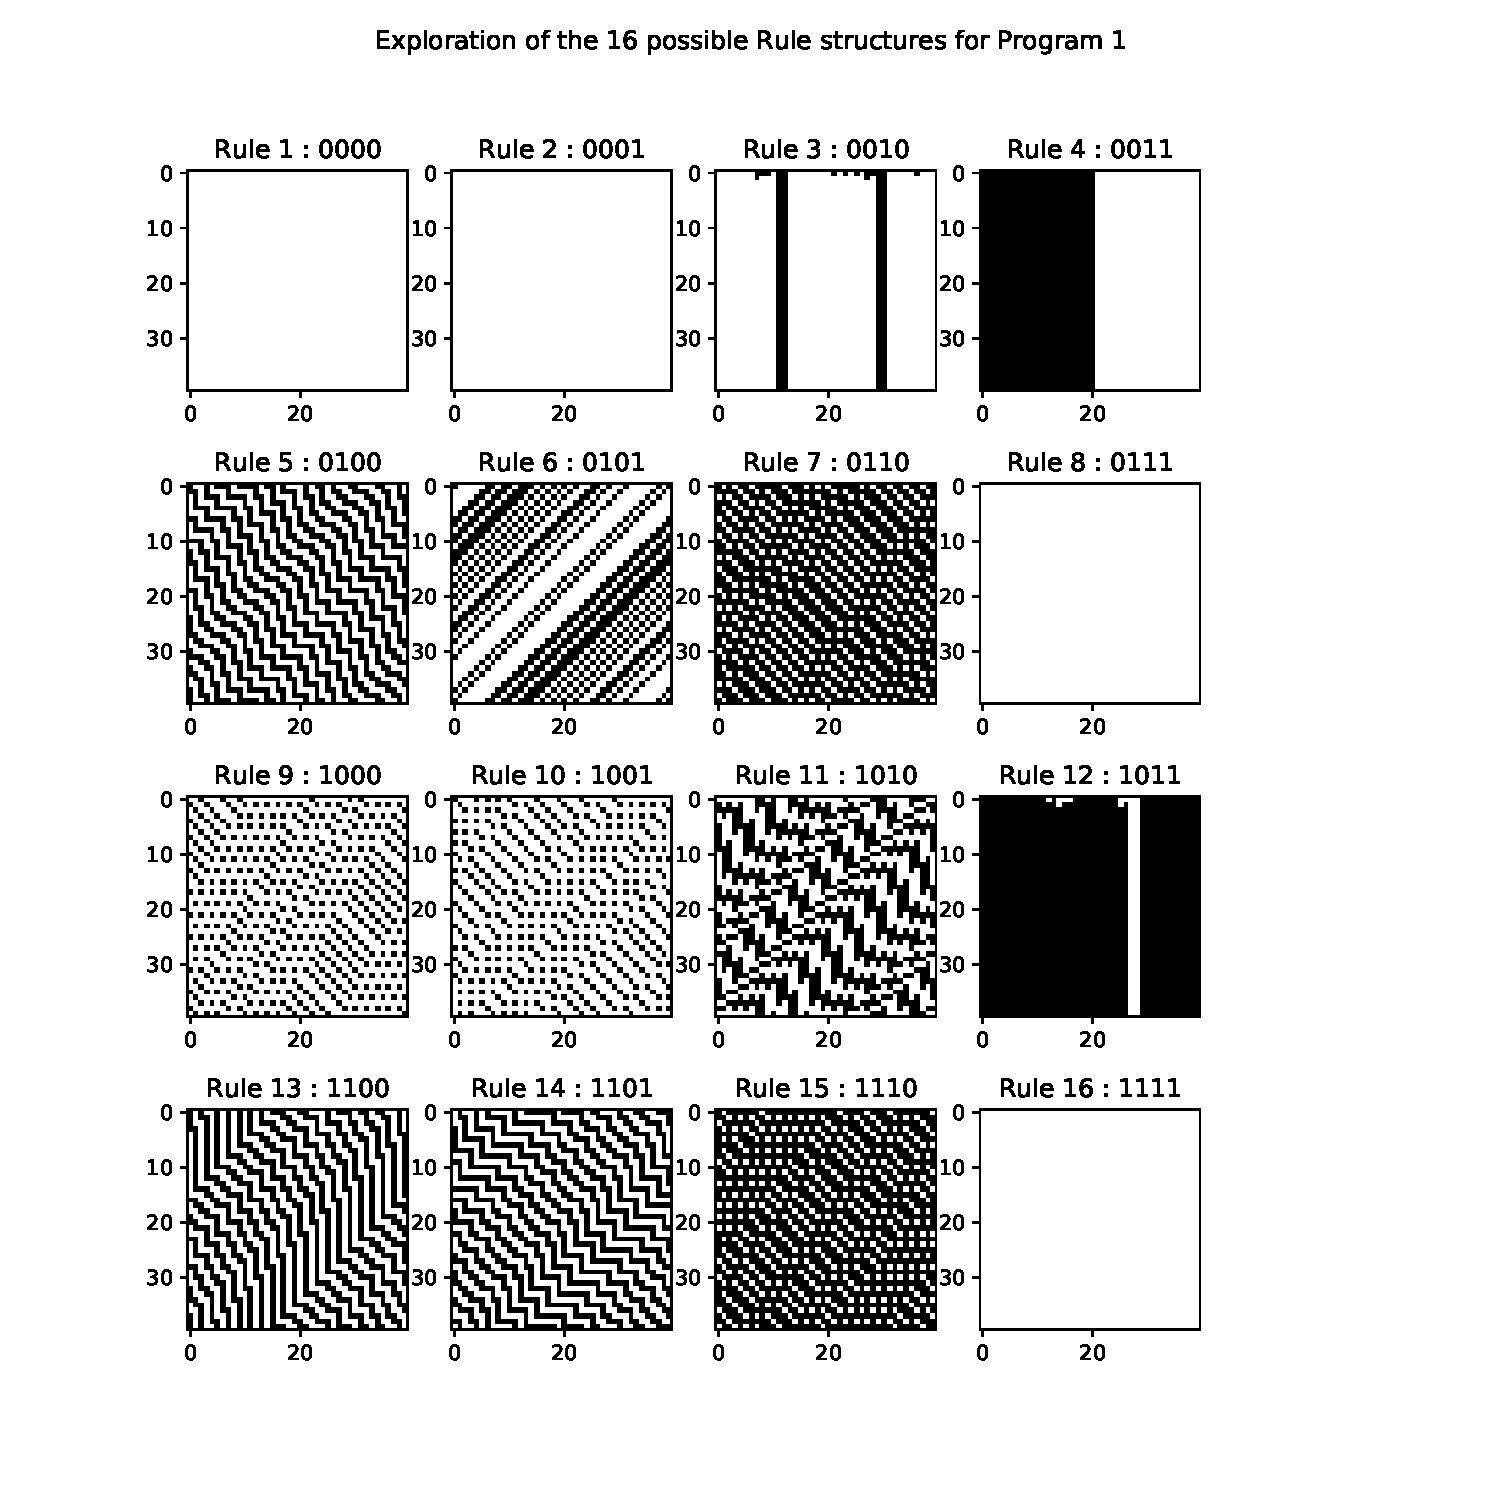
\includegraphics[scale=0.5]{Program 1 Exploration.pdf}
\caption{Implementation of all Program 1 update rules. White = 0, Black = 1. Vertical direction is time}
\end{figure}
\subsection{Discussion}
As can be seen in Figure 1 it seems that for rule 1, 2, 8, and 16 their is no repeating pattern that has risen. Rather it seems that the successive time steps have simply led to the entire automaton being populated with 0s.\\
\\
Rule 3, 4, and 12 all seem to share a property where it seems that initially the cells start to change but quickly reach an equilibrium point where the update rule leads to no change to automaton.\\
\\
Rule 5, 13, and 14 all seem to display a very similar pattern of diagonal 1s and 0s. Where it seems that the pattern is very regular.\\
\\
Rule 9, and 10 also seem to share a regular pattern progression where in general the automaton are populated with 0s but have a repeating sparsely distributed amount of 1s. Quite similar in fact to rule 7, and 15. Except in the latter case we in general have the automaton populated with 1s but have a repeating sparsely distributed amount of 0s. These sparsely distributed cells seem to also follow a diagonal patter.\\
\\
Rule 6, and 11 are the only cases that seem to not share any similarities with other rules. Rule 6 is following a leftward shifting pattern every time step leading to another vertical pattern, but much stronger in regularity compared to the other rules. Rule 11 seems to have a similar progression to rule 5, 13, and 14 but with the irregularities in the diagonals being much more present.\\
\\
What all these automaton seem to show is that any slight change in an update rule can have a dramatic effect on how an automaton progresses in time.\\
\\
If I had more time with this project I believe that exploring all initial automaton configurations would be a good way to see how and if the the initial state may have an effect on the patterns we observe in these automaton currently.
\section{Program 2}
\subsection{Introduction}
After looking at Program 1 it is time now to expand our rule definition. Our aim in this section is to extend the system by allowing it to look more than one step back in time, and allowing it to involve more distant neighbours. Our other aim in this section was to try to find examples that show very regular behaviour and examples that look almost random \cite{proj}. In the following two simulations we will be using a 1 dimensional automaton with 100 cells and will be iterating over 100 time steps. 

\subsection{Program 2.1, Spatial Extension}
In this program we are going to allow the system to look one more spatial step and have a similar update rule to that of our Program 1. In this case we take the remainder when divided by 2 of the sum of $p-2$, $p-1$, $p$ and $p+1$, where $p$ is denoting the coordinate of the cell.\\
\\
In Figure \ref{fig:prog21} we are able to see a randomly behaving automaton. This is likely due to the lack of symmetry in our rule definition which has led to, at least to the human eye, a random pattern. It may well be possible that this pattern is not as random as we think though. Many random number generators developed in previous decades have turned out to be very predictable once enough time was spent analysing them. If I had more time I think I could possible try and analyse this rule possibly to see if the pattern, that is inherit to any random number generator, could be found.
\begin{figure}[H]
\centering
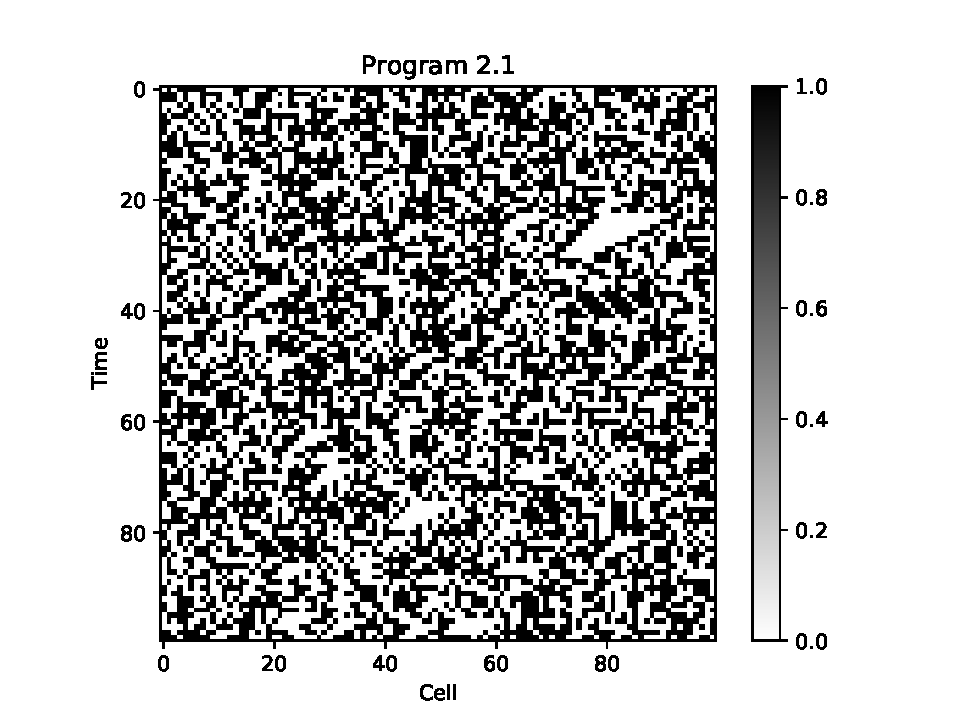
\includegraphics[scale=0.6]{program21.pdf}
\caption{Spatial Extension}\label{fig:prog21}
\end{figure}

\subsection{Program 2.2, Temporal Extension}
In this case we are going to allow the system to look one more temporal step and have a similar update rule to that of our Program 1. In this case we take the remainder when divided by 2 of the sum of $p-1$, $p$, $p+1$ and $p_b+1$. Where $p_b+1$ is the value of the CA at cell $p+1$ from the previous time step.\\
\\
As you can below in Figure \ref{fig:prog22} we are able to see a regularly behaving automaton. This is quite a strange result to come upon. It is not directly obvious that we would see this type of behaviour from a non-symmetrically defined rule. The triangular pattern seems to show a very similar behaviour to that a fractal. It also bares similarity to Stephen Wolfram's Rule 30 \cite{rule30}, which is a famous automaton baring great similarity to Program 2.2.
\begin{figure}[H]
\centering
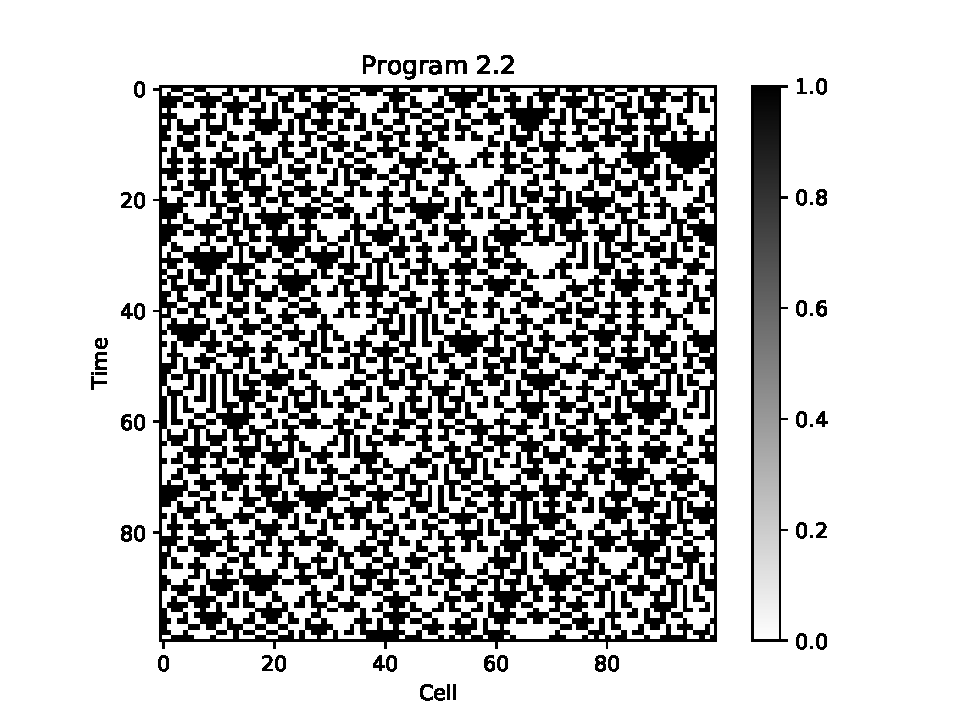
\includegraphics[scale=0.6]{program22.pdf}
\caption{Temporal Extension}\label{fig:prog22}
\end{figure}

\section{Program 3, Conway's Game of Life}
\subsection{Introduction}
Conway's Game of Life is most likely the most famous cellular automaton ever. It was developed by John Horton Conway in 1970 \cite{conway}. I have developed in Python my own implementation of The Game of Life. This has been with the aim of seeing what occurs to a randomly generated initial state and a box of live cells at the centre over 1000 time steps. Conway's Game of Life also has 2 spatial dimensions.\\
\\
Conway's Game of Life uses the following set of rules to update the automaton:
\begin{enumerate}
    \item A dead cell with exactly three living neighbours becomes alive.
    \item A living cell with two or three living neighbours remains alive.
    \item In all other cases, the cell becomes (or remains) dead.
\end{enumerate}
In The Game of Life we also define the neighbours of a cell to be the Moore neighborhood definition. Which implies that where all cells touching the the cell in question are it's neighbours including where they only touch at the corners. Meaning the cell has 8 neighbours.\\
\\
The aim of the box of live cells simulation is to try and see if we are able to see the block in the centre ‘glides’ towards the bottom left, with some change in shape allowed.\\
\\
The aim of the randomly generated initial state is to see if we are able to identify any small stable groups of cells.
\subsection{Results and Discussion}
In Figure \ref{fig:box} we are able to see a direct comparison from the first and last time step of the box of live cells simulation. In this scenario I seem to have not been able to notice any ‘glides’ towards the bottom left. This is after running the simulation 20 times with differently configured boxes. What I did notice was that the symmetry in the box generated a very large structure over the first 100 time steps which then was followed by the structure disintegrating and leaving either nothing or an oscillatory system. If I had more time I would likely want to explore this system in more detail and possibly try and devise a way to track where in the automaton their seems to be the most activity. Activity referring to the rate at which cells are changing values.

\begin{figure}[H]
\centering
\begin{subfigure}{.5\textwidth}
    \centering
    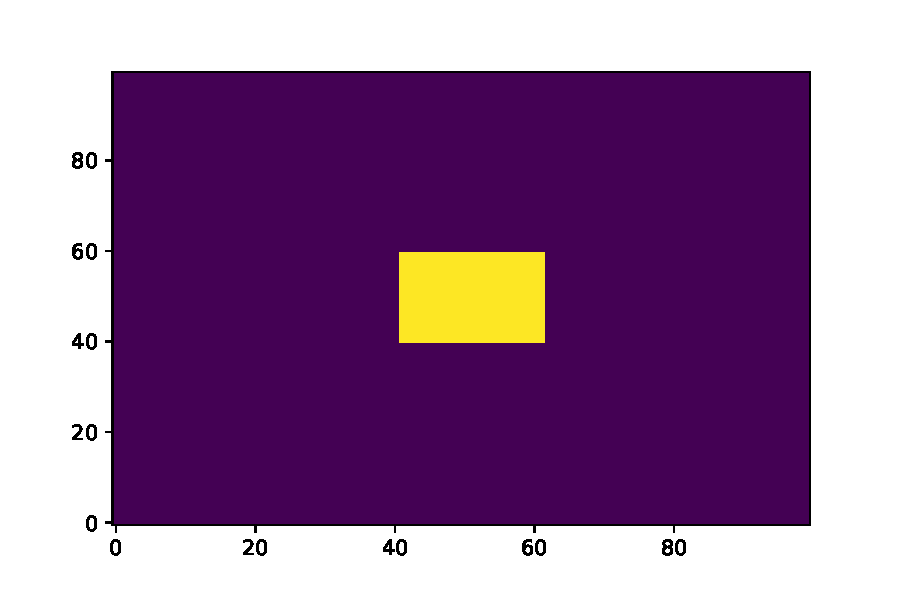
\includegraphics[scale=0.4]{Conway_Box_FIRST.pdf}
    \caption{First time step}\label{fig:box_first}
\end{subfigure}
\begin{subfigure}{.5\textwidth}
    \centering
    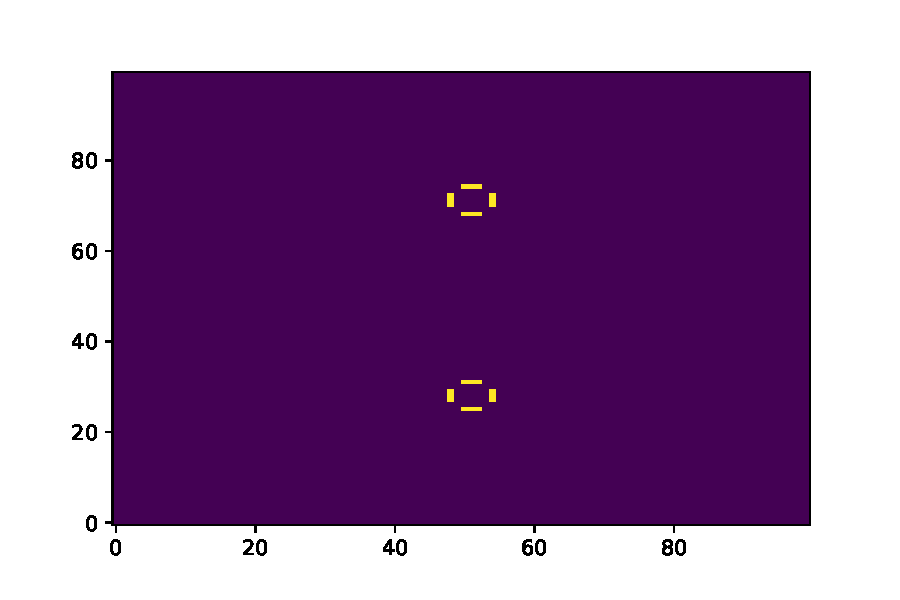
\includegraphics[scale=0.4]{Conway_Box_LAST.pdf}
    \caption{Last time step}\label{fig:box_last}
\end{subfigure}
\caption{Conway's Game of Life with a box of live cells at the centre}\label{fig:box}
\end{figure}

In Figure \ref{fig:ran} we are able to see a direct comparison from the first and last time step of the randomly generated initial state simulation. Comparing the first and last time steps it is clear to see that with the randomly generated initial state we were able to generate small stable groups of cells. These groups of cells are oscillatory systems that have been able to arrive at a point where the number of time steps will not be able to alter the automaton any further since it is now stable. It seems from my observations that a randomly generated initial state usually leads to this type of system, after running this simulation also 20 times. 

\begin{figure}[H]
\centering
\begin{subfigure}{.5\textwidth}
    \centering
    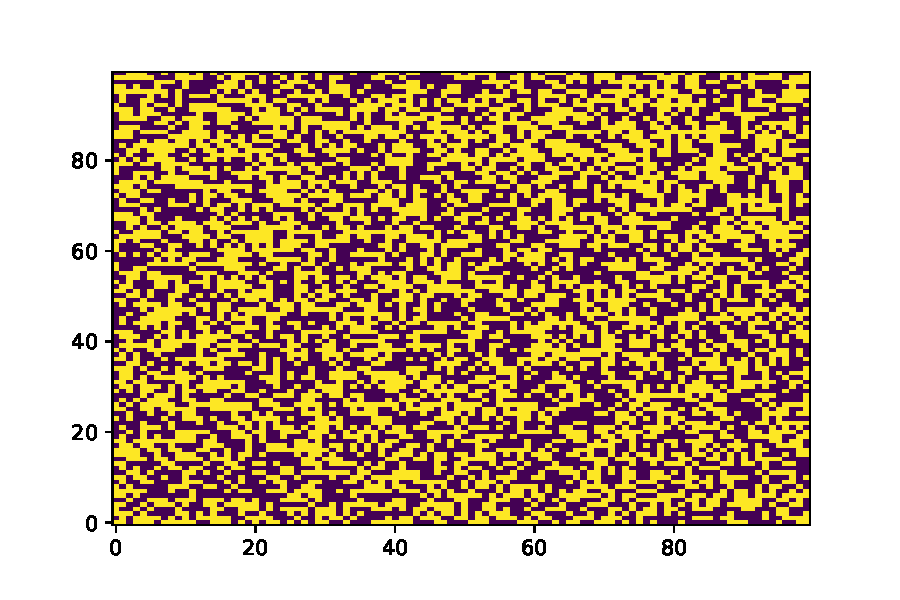
\includegraphics[scale=0.4]{Conway_Random_first.pdf}
    \caption{First time step}\label{fig:ran_first}
\end{subfigure}
\begin{subfigure}{.5\textwidth}
    \centering
    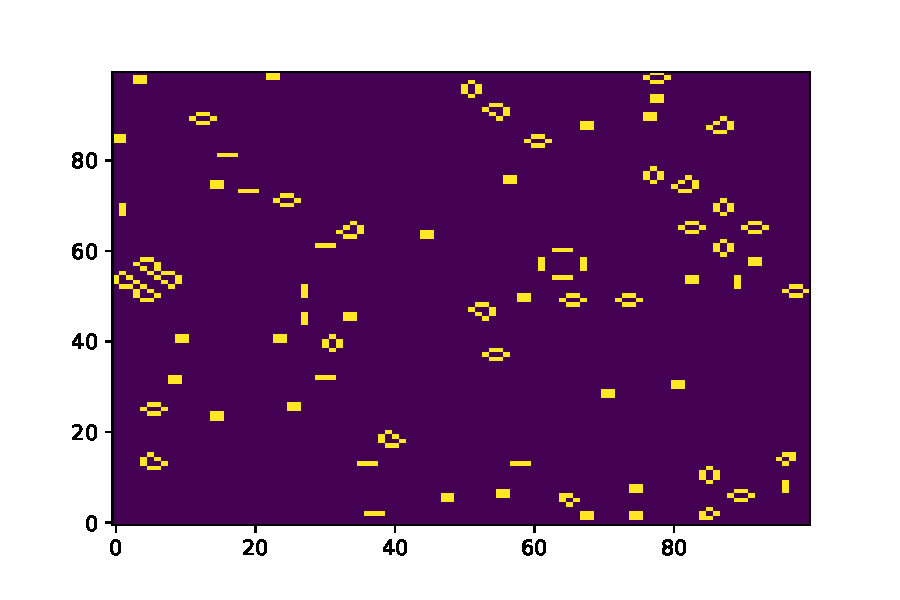
\includegraphics[scale=0.4]{Conway_Random_last.pdf}
    \caption{Last time step}\label{fig:ran_last}
\end{subfigure}
\caption{Conway's Game of Life with a randomly generated initial state}\label{fig:ran}
\end{figure}

\section{Program 4, Forest Fire Simulation}
\subsection{Introduction}
In this program we will be simulating a forest fire, where one inputs an initial cellular automata which is representative of the forest. In this simulation we have 3 values which a cell is able to take:
\begin{itemize}
  \item $0$ = burnt-out/dead forest
  \item $1$ = green/live forest
  \item $2$ = burning forest
\end{itemize}
The following rules apply in this automaton:
\begin{enumerate}
    \item A burnt-out/dead ($0$) forest sprouts green/live forest with a probability $p$ per cell per time step.
    \item If a cell is burning ($2$), then in the next time step any neighbouring cell that were previously green/live forest ($1$) will catch fire.
    \item A burning ($2$) cell that was alight will become burnt-out/dead ($0$) forest in the next time step.
    \item Lightning may strike, allowing any green/live ($1$) forest cell to catch fire becoming burning ($2$) forest with probability $f$ per cell per time step.
\end{enumerate}{}
In this simulation we are also going to be using the Von Neumann neighborhood as our way of defining the value of our $(i, j)$ cell. Which implies that where all cells touching the the cell in question are it's neighbours but not including where they only touch at the corners. Meaning the cell has 4 neighbours.\\
\\
The first aim of this program is to run an initial simulation being where we explore how fires propagate through a 100 by 100 cell forest for 100 time steps. Where we will set our parameters as:
$$
p = 0.05
$$
$$
f = 0.00025
$$
With a forest containing no fires but with 30\% of the cells occupied by green/alive forest, in the centre.

\subsection{Results of Initial Simulation}
The results of the initial simulation are very promising and show some sign of regular behaviour. As can be seen in Figure \ref{fig:initial_fire} their seems to be a an oscillatory behaviour occurring with the number of live and dead cells over the course of the whole simulation. It is as if the values are experiencing some form of damping also. As is clear in the graph we can notice that the values are mirroring each other around a common equilibrium value. In order to see more clearly what is happening we will now look at the next program where we have run many more simulations.

\begin{figure}[H]
\centering
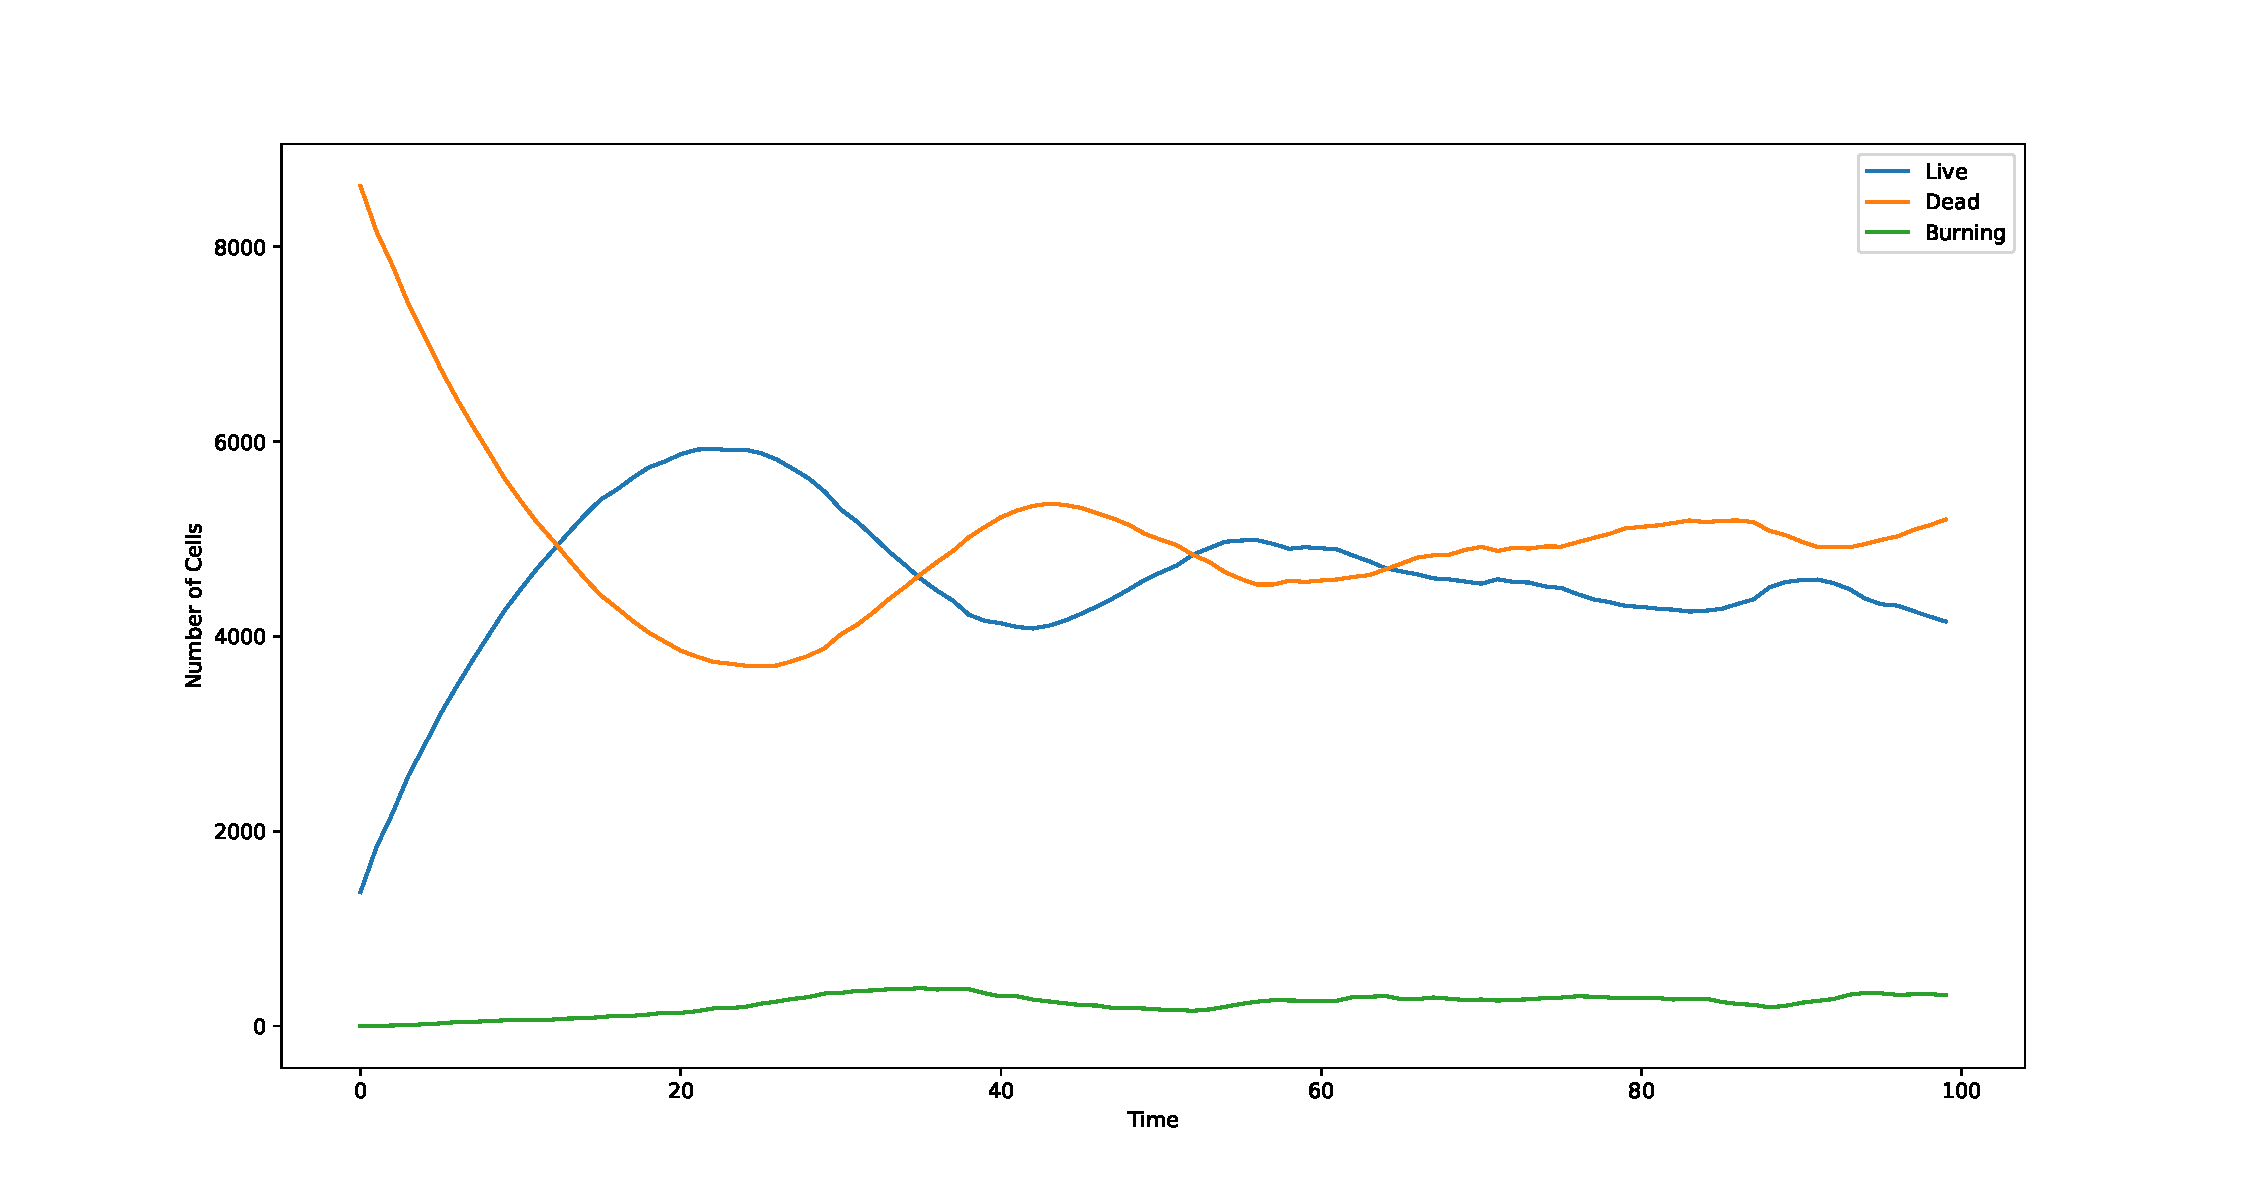
\includegraphics[scale=0.3]{Initial Forest Fire.pdf}
\caption{Initial Forest Fire Simulation}\label{fig:initial_fire}
\end{figure}

\subsection{Large Scale Simulation}
In this section we will be discussing the results that have arisen from 2 large scale simulations which I ran in order to see more clearly the variations in behaviour of the forest fire when we are varying the $p$ and $f$ values. To do this I ran 2 large scale simulations which compromised of 441 simulations each. The first one used the following values for the simulation:
$$
p = (0.001, 0.05, 0.1, 0.15, 0.2, 0.25, 0.3, 0.35, 0.4, 0.45, 0.5, 0.55, 0.6, 0.65, 0.7, 0.75, 0.8, 0.85, 0.9, 0.95, 0.99)
$$
$$
f = (0.00025, 0.05, 0.1, 0.15, 0.2, 0.25, 0.3, 0.35, 0.4, 0.45, 0.5, 0.55, 0.6, 0.65, 0.7, 0.75, 0.8, 0.85, 0.9, 0.95, 0.999)
$$
\\
Below I have created multiple plots in order to illustrate the data generated by the simulations. I had noticed after running multiple values for $p$ and $f$ that the oscillatory behaviour occurring was not unique to the initial configuration but instead was the normal, which is expected when one thinks about what the rules stated above imply. To try and quantify this data in a more manageable way I created scalar plots which illustrate the mean and standard deviation for the live, dead, and burning cells of all the $p$ and $f$ values detailed above. I also created surface plots to try and give more ways of visualising the data I had gathered.\\
\\
As you can see in Figure \ref{fig:live} the live mean seems to show that as the $p$ value increase and the $f$ value decreases their is an increase in the mean number of live cells. It also shows that in general as the $p$ value decreases and the $f$ value increases their is a decrease in the standard deviation of the number of live cells.
\begin{figure}[H]
\centering
\begin{subfigure}{.5\textwidth}
    \centering
    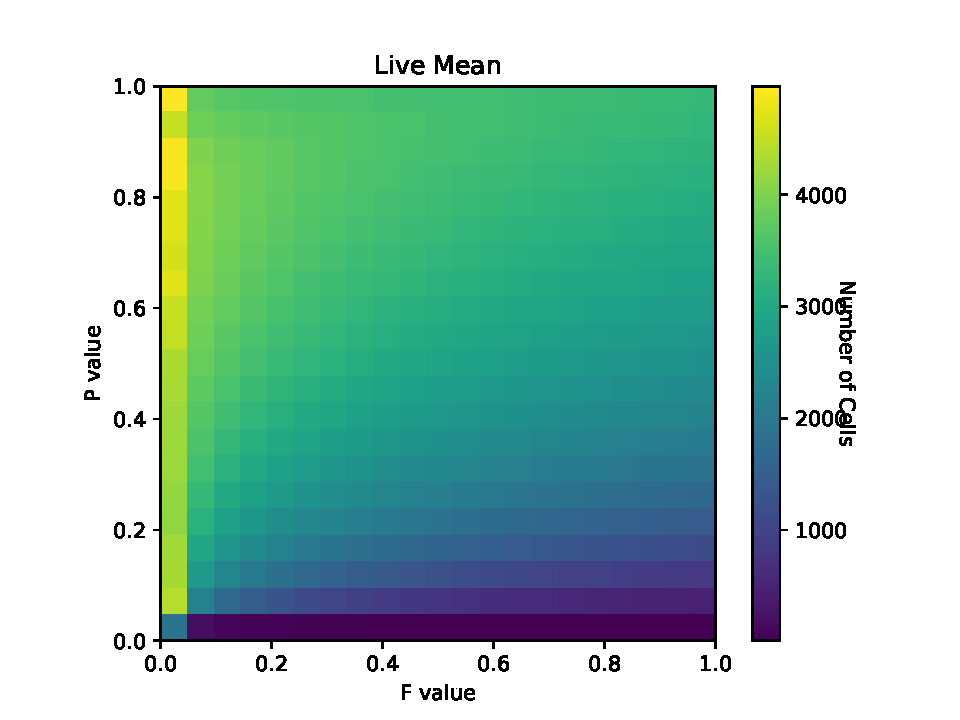
\includegraphics[scale=0.4]{Live Mean.pdf}
    \label{fig:livemean}
\end{subfigure}%
\begin{subfigure}{.5\textwidth}
    \centering
    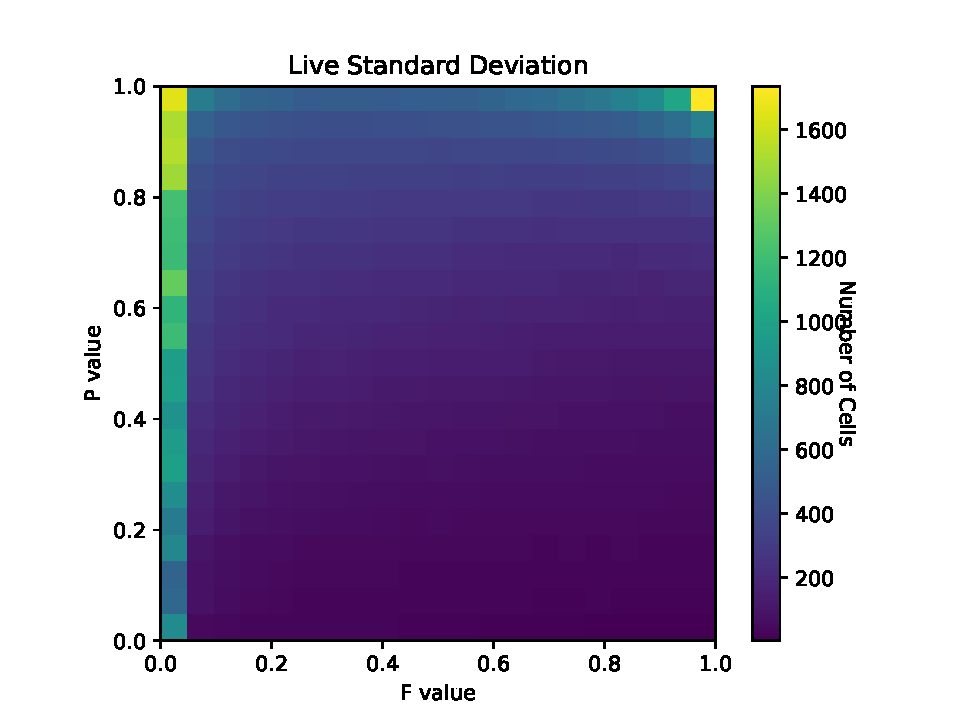
\includegraphics[scale=0.4]{Live STD.pdf}
    \label{fig:livestd}
\end{subfigure}
\label{fig:live}
\end{figure}
\begin{figure}[H]
\centering
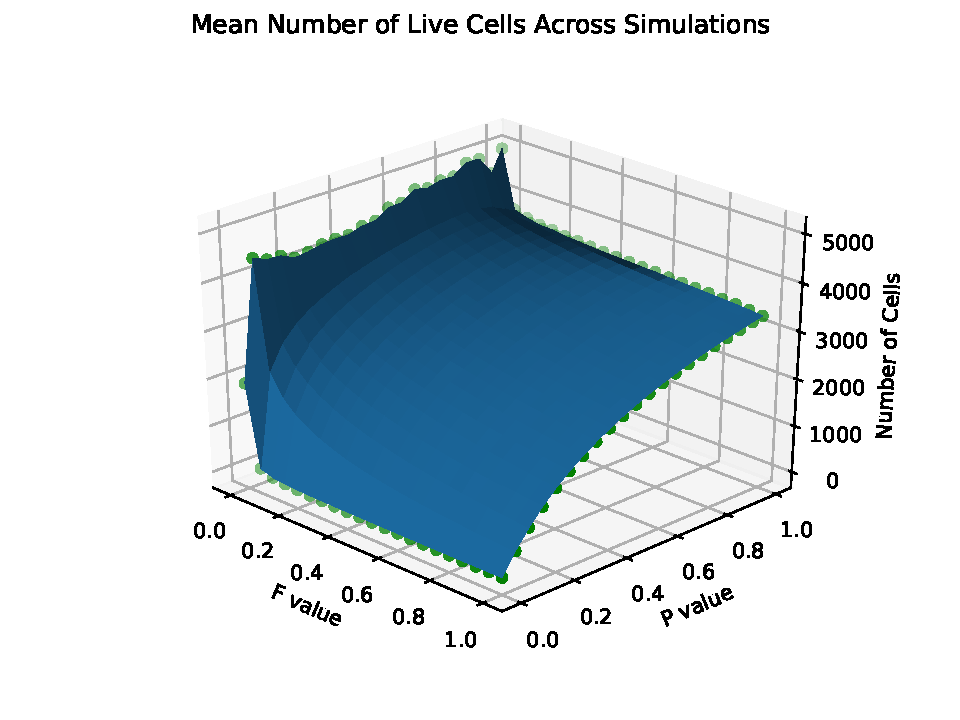
\includegraphics[scale=0.6]{Live Mean 3D.pdf}
\label{fig:livemean3D}
\end{figure}
As you can see in Figure \ref{fig:dead} the dead mean seems to show that as the $p$ value increase their is a decrease in the mean number of dead cells. In general it seems that the p and f values do not have any significance in the standard deviation of the number of dead cells.
\begin{figure}[H]
\centering
\begin{subfigure}{.5\textwidth}
    \centering
    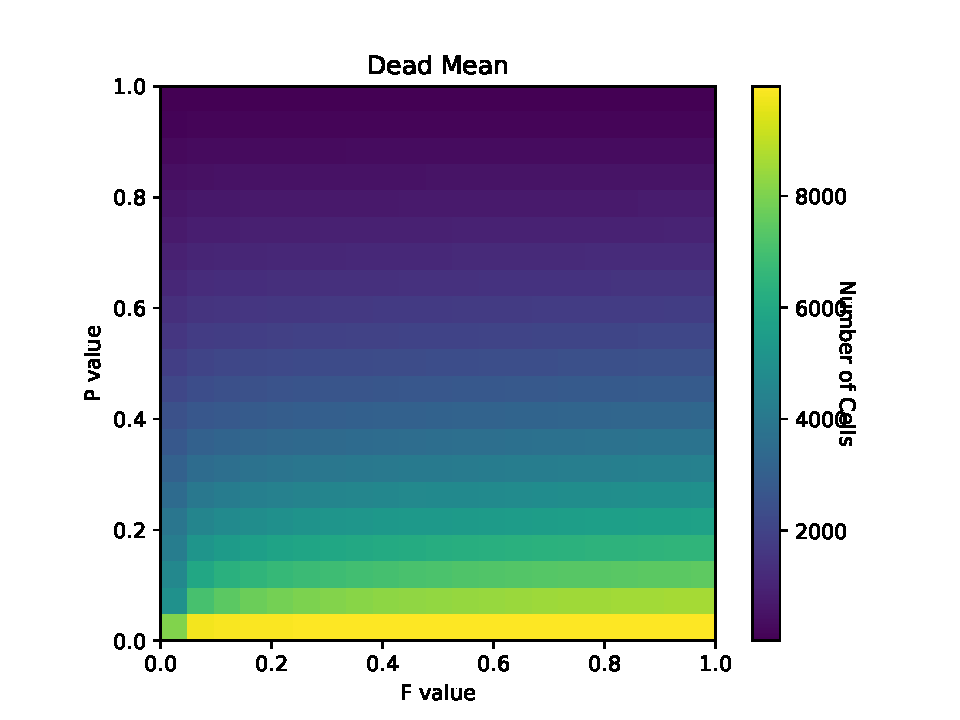
\includegraphics[scale=0.4]{Dead Mean.pdf}
    \label{fig:deadmean}
\end{subfigure}%
\begin{subfigure}{.5\textwidth}
    \centering
    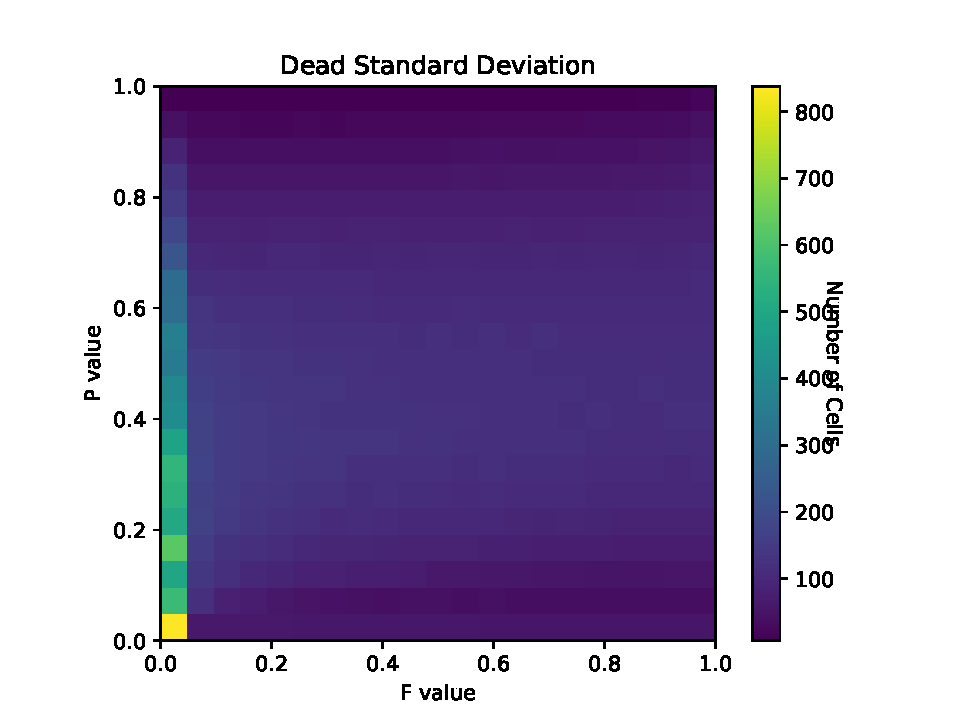
\includegraphics[scale=0.4]{Dead STD.pdf}
    \label{fig:deadstd}
\end{subfigure}
\label{fig:dead}
\end{figure}
\begin{figure}[H]
\centering
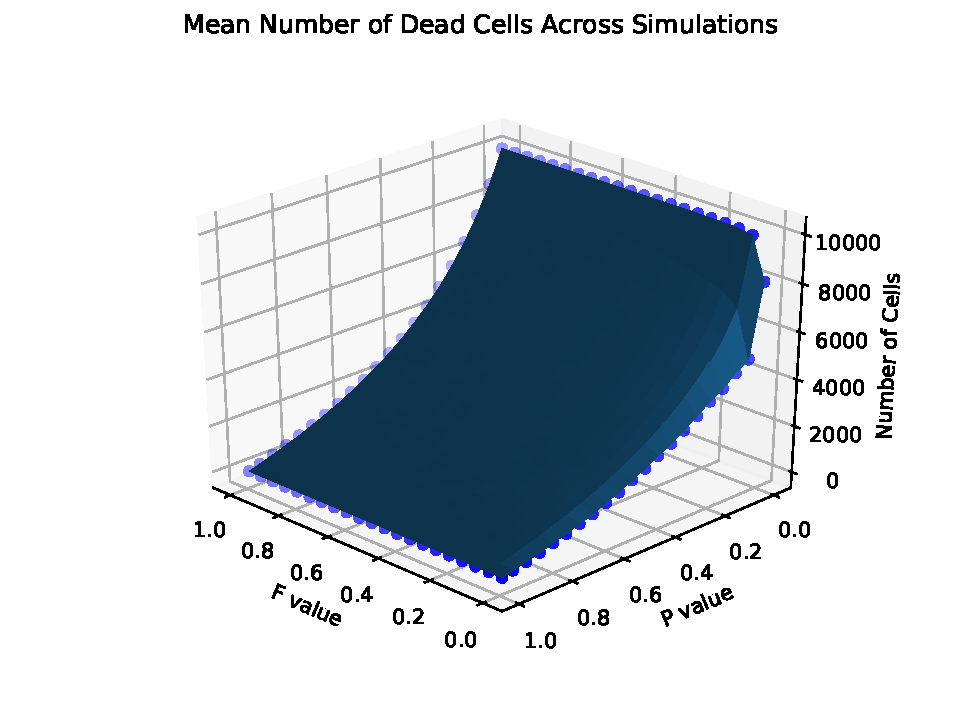
\includegraphics[scale=0.6]{Dead Mean 3D.pdf}
\label{fig:deadmean3D}
\end{figure}
As you can see in Figure \ref{fig:burn} the burning mean seems to show that as the $p$ value increase their is an increase in the mean number of burning cells. In general it seems that the p and f values do not have any significance in the standard deviation of the number of burning cells.
\begin{figure}[H]
\centering
\begin{subfigure}{.5\textwidth}
    \centering
    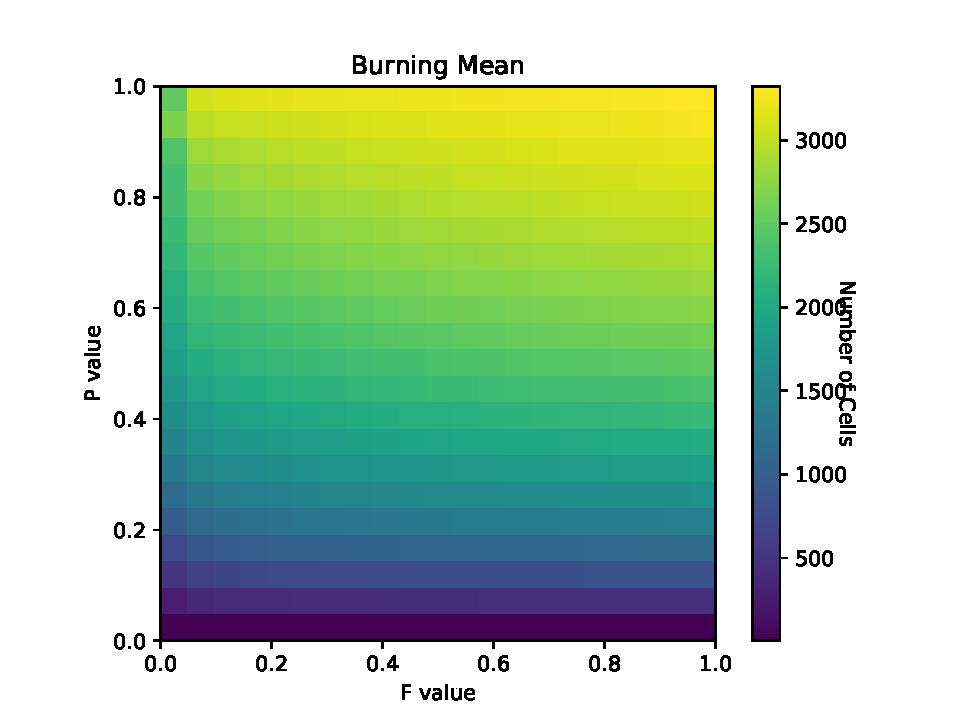
\includegraphics[scale=0.4]{Burning Mean.pdf}
    \label{fig:burnmean}
\end{subfigure}%
\begin{subfigure}{.5\textwidth}
    \centering
    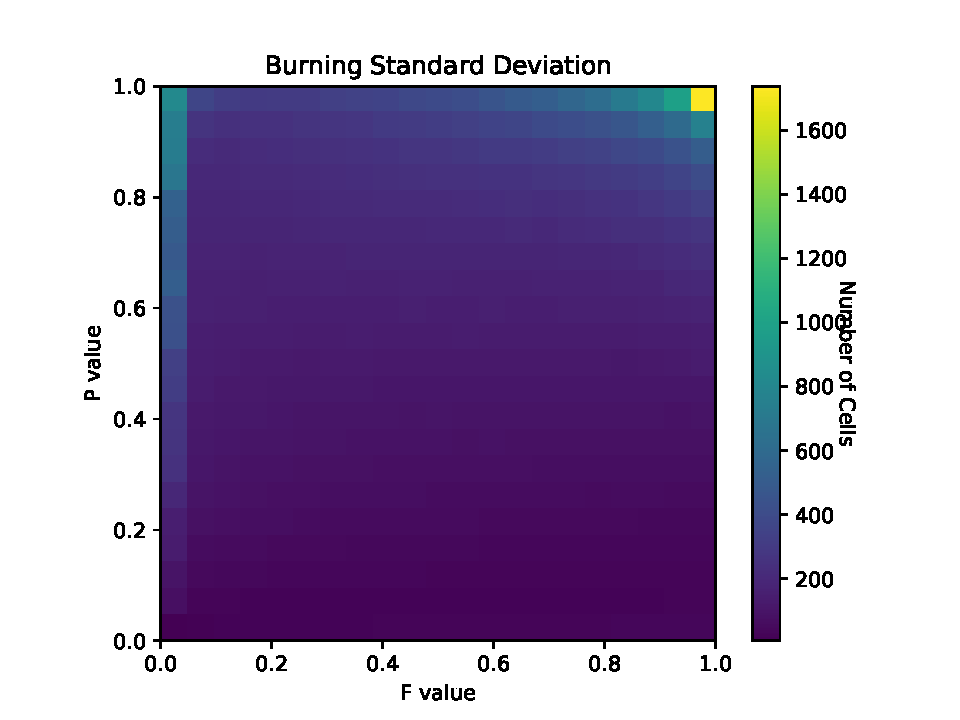
\includegraphics[scale=0.4]{Burning STD.pdf}
    \label{fig:burnstd}
\end{subfigure}
\label{fig:burn}
\end{figure}
\begin{figure}[H]
\centering
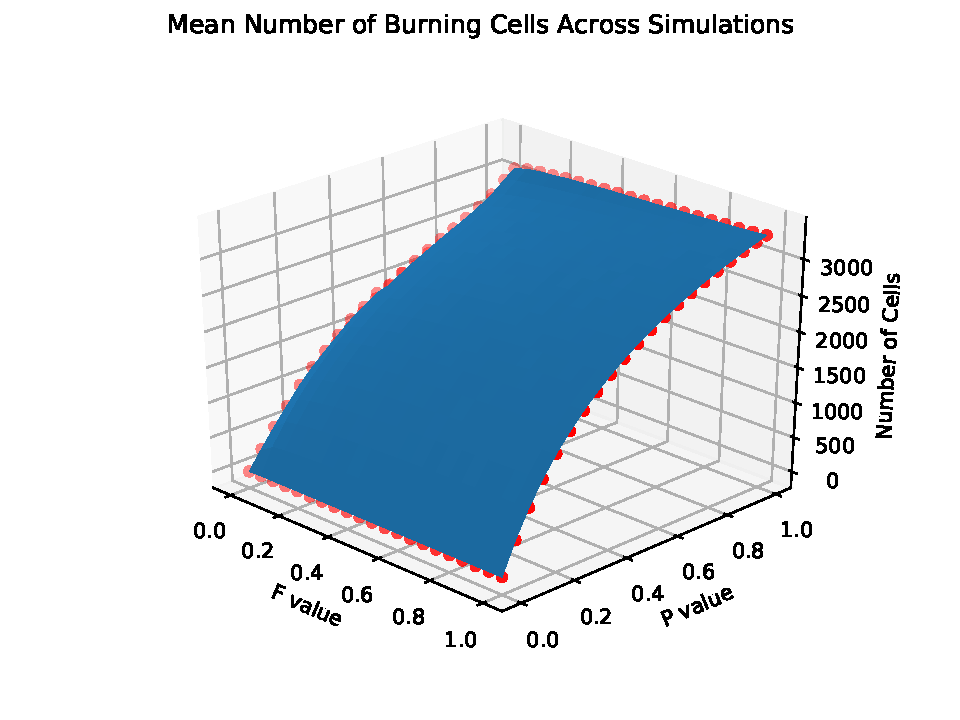
\includegraphics[scale=0.6]{Burning Mean 3D.pdf}
\label{fig:burnmean3D}
\end{figure}
As can be seen quite clearly though their seems to be a discontinuity in the general trends at the lowest $f$ value column of data. This made me inquire over the possibility that their maybe some more relationships towards these lower values which would be interesting to explore.\\
\\
In order to this I ran a second simulation which covered the following $p$ and $f$ values:\\
\\
$p$ = (0.001, 0.05, 0.1, 0.15, 0.2, 0.25, 0.3, 0.35, 0.4, 0.45, 0.5, 0.55, 0.6, 0.65, 0.7, 0.75, 0.8, 0.85, 0.9, 0.95, 0.99)\\
\\
$f$ = (1.0e-05, 5.0e-05, 1.0e-04, 1.5e-04, 2.0e-04, 2.5e-04, 3.0e-04, 3.5e-04, 4.0e-04, 4.5e-04, 5.0e-04, 5.5e-04, 6.0e-04, 6.5e-04, 7.0e-04, 7.5e-04, 8.0e-04, 8.5e-04, 9.0e-04, 9.5e-04, 1.0e-03)\\
\\
The new plots generated for these $p$ and $f$ values are featured below this text.
\begin{figure}[H]
\centering
\begin{subfigure}{.5\textwidth}
    \centering
    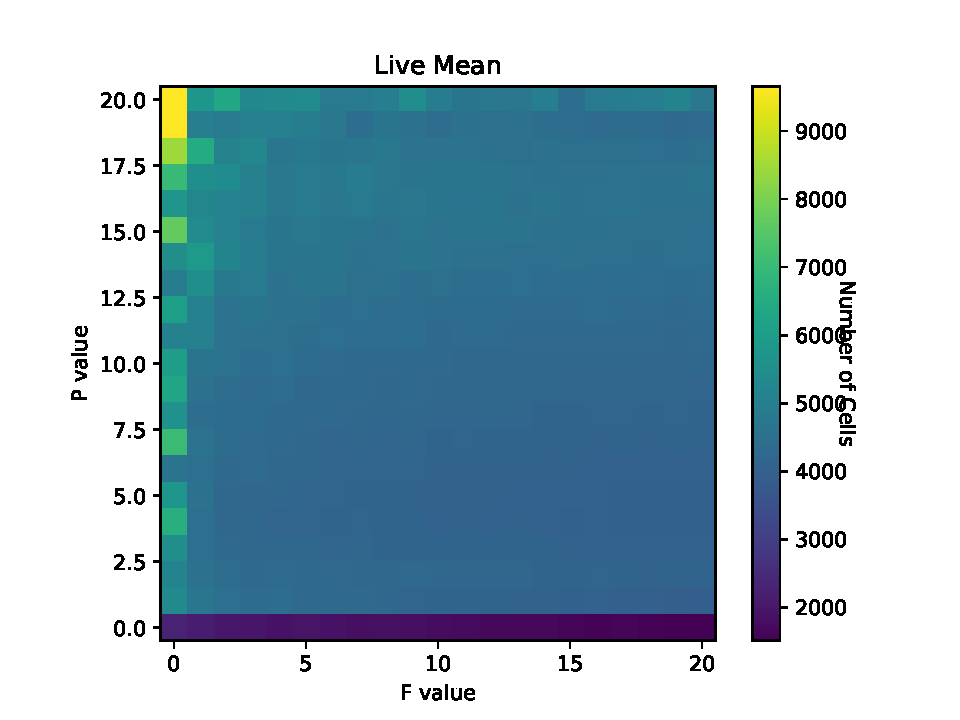
\includegraphics[scale=0.4]{Live Mean 2.pdf}
    \label{fig:livemean3D}
\end{subfigure}%
\begin{subfigure}{.5\textwidth}
    \centering
    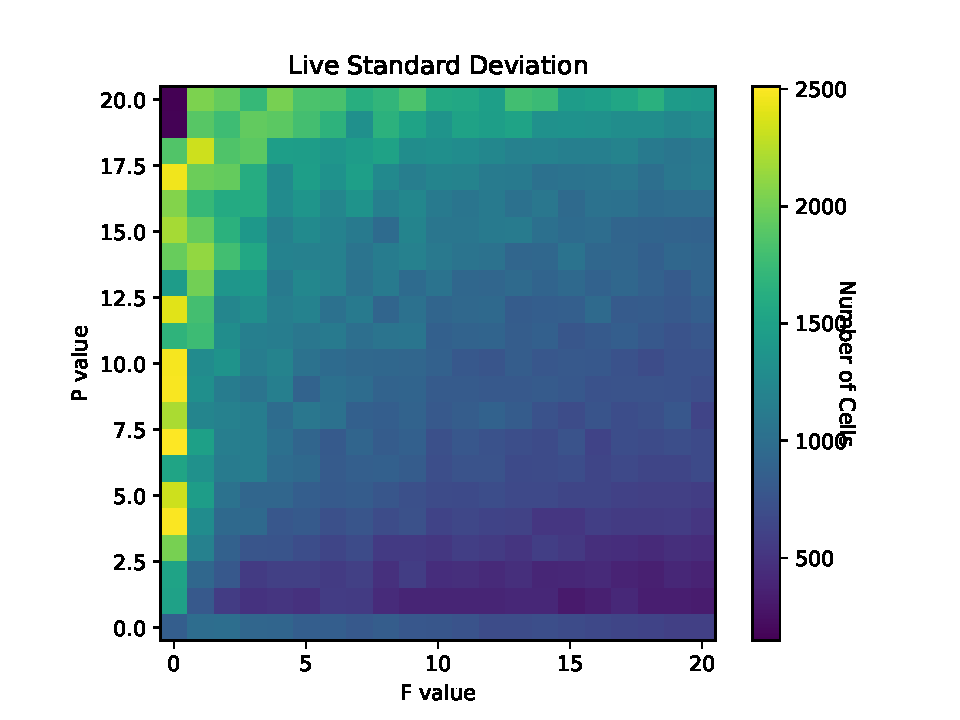
\includegraphics[scale=0.4]{Live STD 2.pdf}
    \label{fig:livestd}
\end{subfigure}
\end{figure}
\begin{figure}[H]
\centering
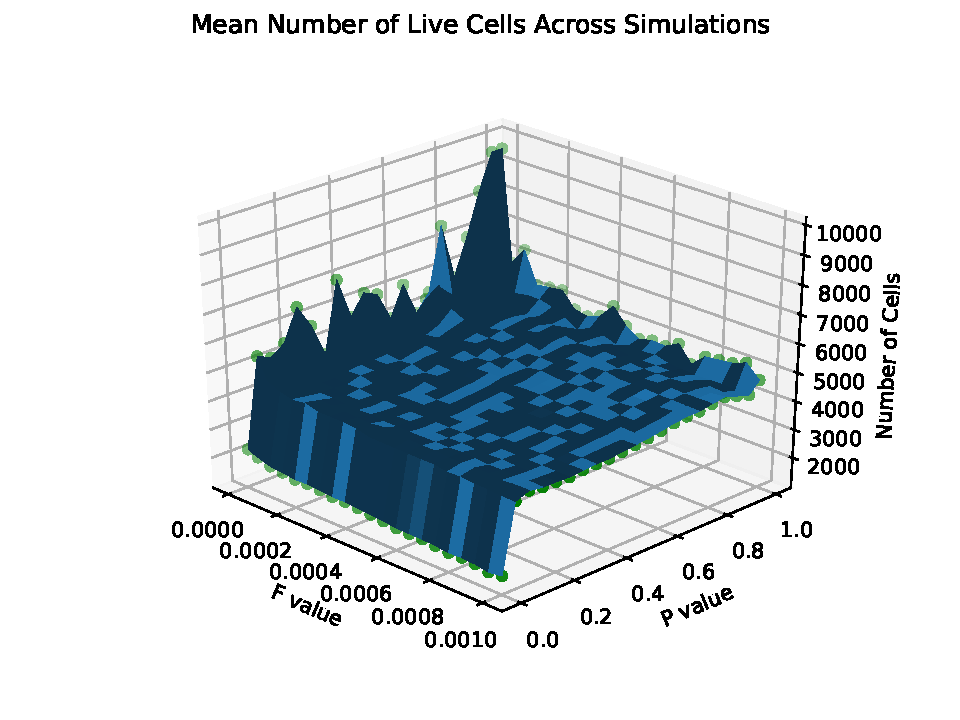
\includegraphics[scale=0.6]{Live Mean 3D 2.pdf}
\label{fig:livemean3D}
\end{figure}

\begin{figure}[H]
\centering
\begin{subfigure}{.5\textwidth}
    \centering
    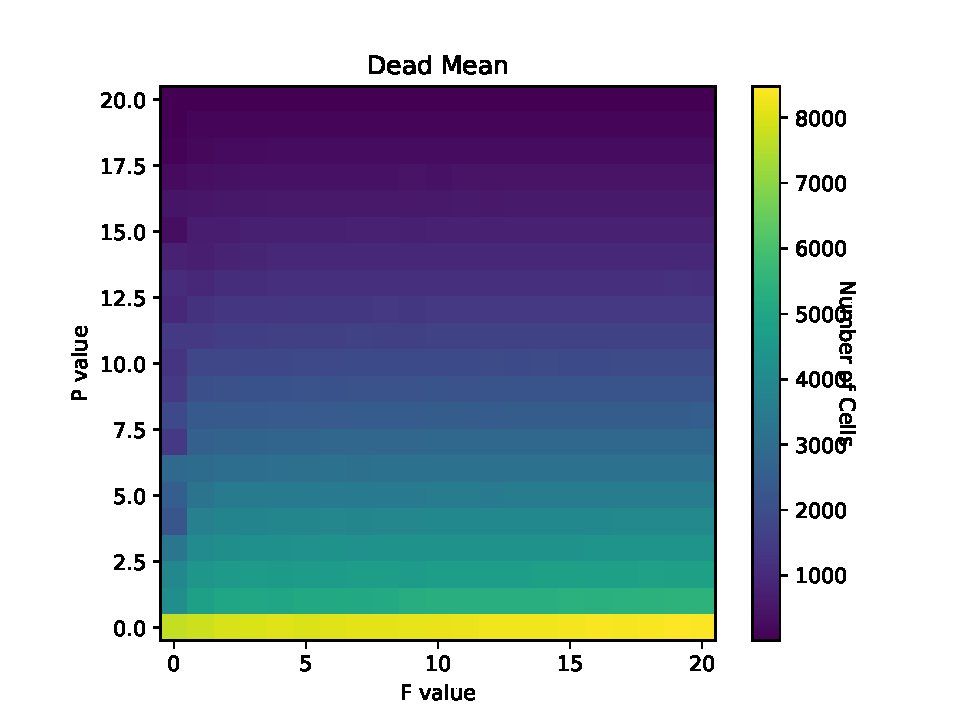
\includegraphics[scale=0.4]{Dead Mean 2.pdf}
    \label{fig:livemean3D}
\end{subfigure}%
\begin{subfigure}{.5\textwidth}
    \centering
    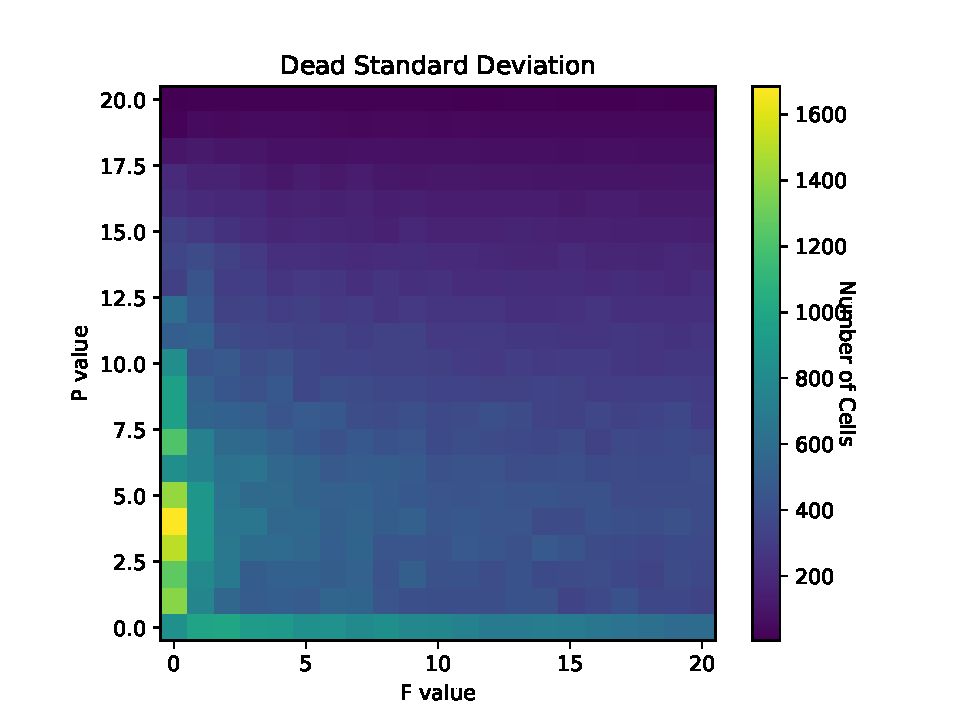
\includegraphics[scale=0.4]{Dead STD 2.pdf}
    \label{fig:livestd}
\end{subfigure}
\end{figure}
\begin{figure}[H]
\centering
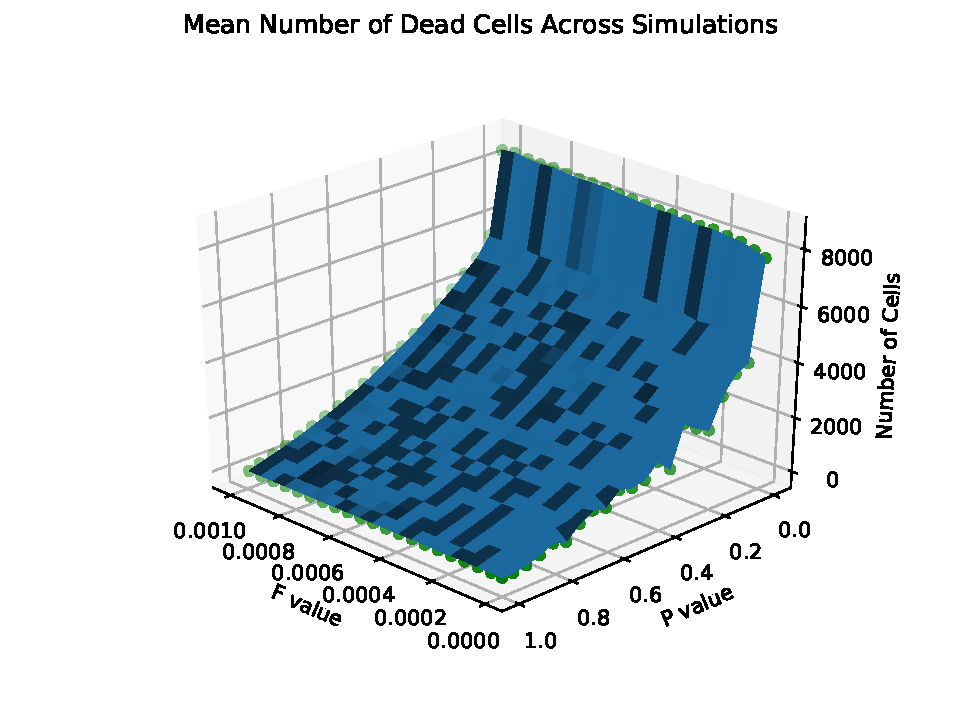
\includegraphics[scale=0.6]{Dead Mean 3D 2.pdf}
\label{fig:deadmean3D}
\end{figure}

\begin{figure}[H]
\centering
\begin{subfigure}{.5\textwidth}
    \centering
    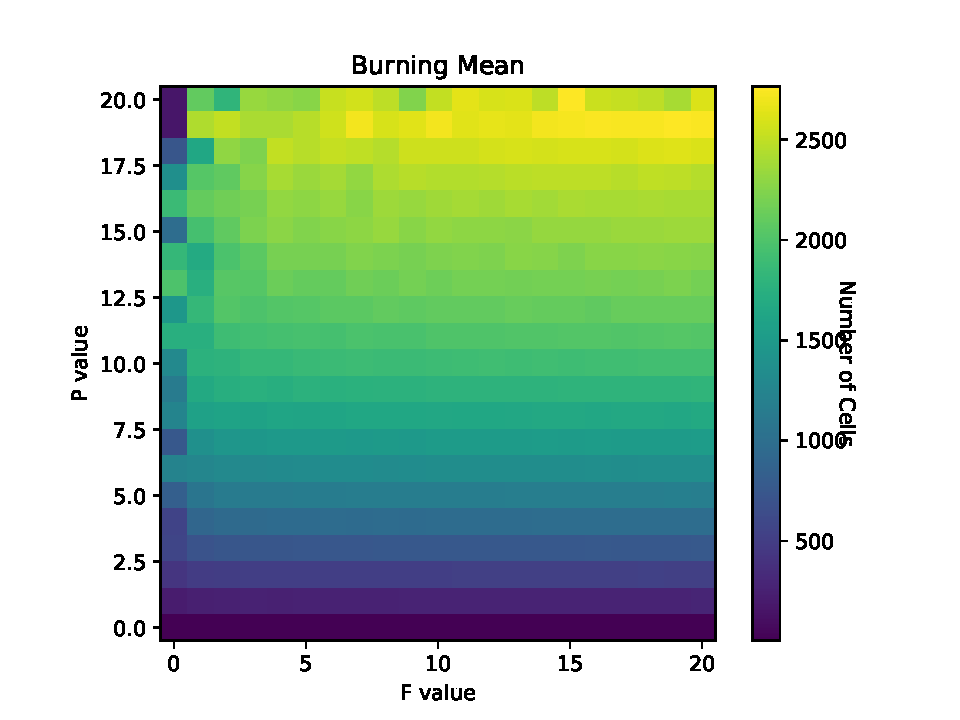
\includegraphics[scale=0.4]{Burning Mean 2.pdf}
    \label{fig:livemean3D}
\end{subfigure}%
\begin{subfigure}{.5\textwidth}
    \centering
    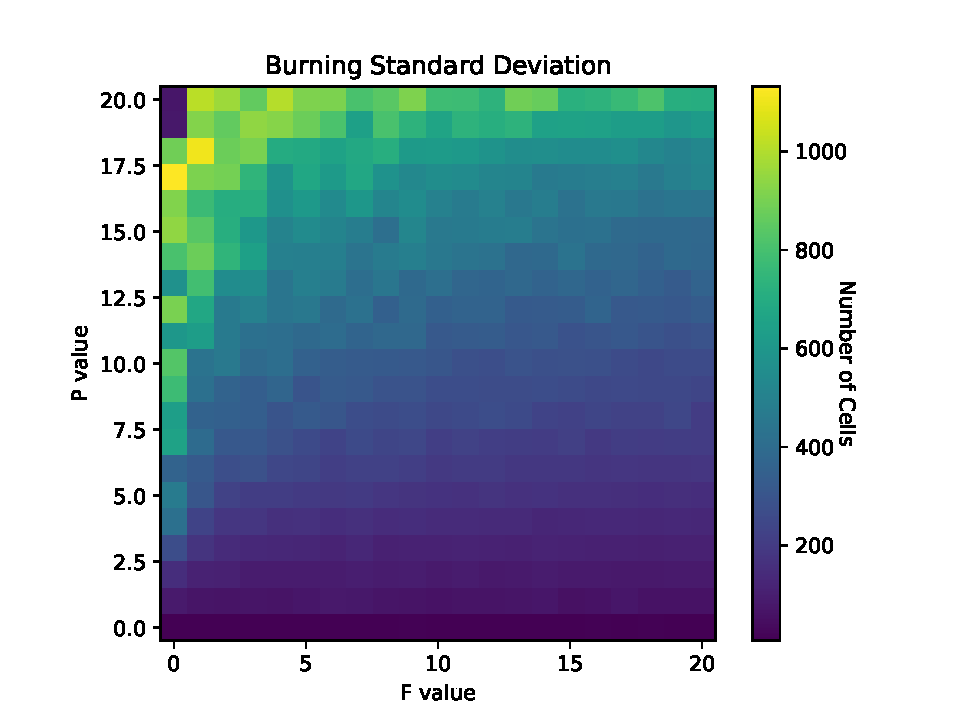
\includegraphics[scale=0.4]{Burning STD 2.pdf}
    \label{fig:livestd}
\end{subfigure}
\label{fig:live}
\end{figure}
\begin{figure}[H]
\centering
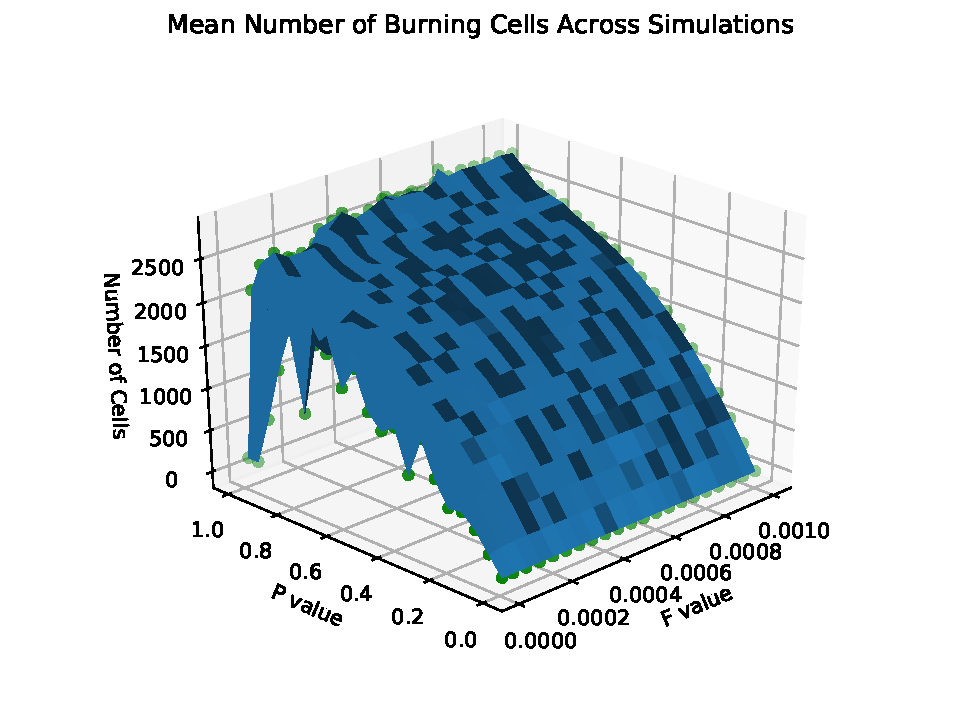
\includegraphics[scale=0.6]{Burning Mean 3D 2.pdf}
\label{fig:burnmean3D}
\end{figure}
\subsection{Discussion and Conclusion}
Looking over all these plots and comparing them to the corresponding plots from the first simulation it seems as though my initial enquiry over the lower $f$ values has had some mixed outcomes. It seems as though the general patterns observed on the larger scale still do stay true. Although their does seem to be some variation in the data compared to the previous large scale. Comparing the corresponding surface plots to each other it is very clear to see that the initial relationships suggested by the first simulation have stayed very similar. The surface plots do seem to have acquired an element of volatility though which is not fully understood from where. This is most clearly shown in the Mean Burning Cells and Live Cells surface plots which towards the lower $f$ values have once again shown a great amount of discontinuity when compared to the rest of the surface plot. This may be indicative that a further simulation could be done in order to try and probe this phenomena further. I would say that that would likely be one of the highest priority tasks I would want to accomplish if given more time.\\
\\
Looking at the scalar plots more closely though you can that in the live mean and standard deviation plots from the first simulation compared to the second simulation the range of values which the standard deviation holds is much wider the second simulation, ranging from 2500 to 300 roughly, whilst in the first simulation we see the values ranging from 1600 to 100. The live mean has also drastically increased from having a mean value of 2500 to 6000 in the second simulation. The dead cells plots seem to have stayed quite consistent except we have now found a simulation, once again around the lower $f$ values, where the standard deviation has gone to roughly 1600, double that of the highest value from the first simulation.\\
\\
The burning scalar plots seem to have been affected the most in terms of appearance from the comparison between the two simulations. Where they now contain many more irregularities in the overall relationship compared to the first simulation.\\
\\
In conclusion, I think that if I had more time I would have liked to preform a further simulation perhaps even running multiple of the same simulation to try and get more statistically accurate data by spreading the possible errors which may be arising over multiple simulations. I would have also liked to have possibly tried to see if the initial configuration of a forest changes how the forest fire evolves. My theory would be that in general it would not. This is an extrapolation though from the data I saw in Program 1. 
\bibliographystyle{plain}
\bibliography{refs}

\end{document}
